%%This is a very basic article template.
%%There is just one section and two subsections.
\documentclass[a4paper,10pt]{article}
\usepackage[utf8]{inputenc}
\renewcommand*\rmdefault{phv}
\usepackage{graphicx}
\usepackage{multicol}
%
%%Cria os índices
\usepackage{hyperref}
\hypersetup{colorlinks=true,allcolors=blue}
\usepackage{hypcap}
%
%% 
\usepackage{pdflscape}
\usepackage{capt-of}
%
%%
%%Cofiguração do Java
\usepackage{geometry}
\geometry{margin=.5in}
%% Definiciações de Hightlight para codigos java
\usepackage{listings}
\usepackage{color}

\definecolor{dkgreen}{rgb}{0,0.6,0}
\definecolor{gray}{rgb}{0.5,0.5,0.5}
\definecolor{mauve}{rgb}{0.58,0,0.82}
\definecolor{lightgray}{rgb}{0.96,0.96,0.96}

\lstset{frame=tb,
  backgroundcolor=\color{lightgray},	
  language=Java,
  aboveskip=3mm,
  belowskip=3mm,
  showstringspaces=false,
  columns=flexible,
  basicstyle={\small\ttfamily},
  numbers=left,
  numberstyle=\small\color{gray},
  keywordstyle=\color{blue},
  commentstyle=\color{dkgreen},
  stringstyle=\color{mauve},
  breaklines=true,
  breakatwhitespace=true,
  tabsize=3
}
%% Definiciações de Hightlight para codigos XML
\usepackage{listings}

\usepackage{color}
\definecolor{gray}{rgb}{0.4,0.4,0.4}
\definecolor{darkblue}{rgb}{0.0,0.0,0.6}
\definecolor{cyan}{rgb}{0.0,0.6,0.6}
\definecolor{mauve}{rgb}{0.58,0,0.82}
\definecolor{orange}{rgb}{1.0, 0.49, 0.0}

\lstset{
  basicstyle=\ttfamily,
  columns=fullflexible,
  showstringspaces=false,
  commentstyle=\color{gray}\upshape
}

\lstdefinelanguage{XML}
{
  morestring=[b]",
  morestring=[s]{>}{<},
  commentstyle=\color{orange},
  morecomment=[s]{!--}{--},
  stringstyle=\color{black},
  identifierstyle=\color{darkblue},
  keywordstyle=\color{mauve},
  morekeywords={
  	xmlns,
  	type,
  	styleClass,
  	rendered,
  	layout,
  	id,
  	name,
  	style,
  	widgetVar}% list your attributes here
}  
%
%% 
\usepackage{dirtree}
\newcommand\myicon[1]{{\color{#1}\rule{2ex}{2ex}}}
\newcommand{\folder}[2]{\myicon{#1}\ {#2}}
%%  
%%%
%%%% 
%%%%%
\begin{document}
\title{Layout e Páginas JSF}
\author{José Ribamar Monteiro da Cruz}
\maketitle
\tableofcontents
%
%% Objetivo
%%% 
\section{Objetivo}

O presente documento tem como objetivo apresentar uma proposta de
organização de código para projetos JSF utilizando o conceito de páginas (\emph{pages}).
Tal proposta visa criar uma correlação entre os \textbf{mockups de tela},
os \textbf{códigos java} necessários para montar tal tela bem como os
respectivos \textbf{códigos XHTMLs}.

Juntamento com este conceito (\emph{pages}) é apresentado um forma de criação de
um \textbf{template padrão} configurável que torna a criação de templates xhtml
flexivéis e evita a proliferação de diversos templates pelo projeto que possuam
variações mínimas entre si.
%%%%%%%%%%%%%%%%%%%%%%%%%%%%%%%%%%%%%%%%%%%%%%%%%%%%%%%%%%%%%
% 
%  Introdução 
%
%%%%%%%%%%%%%%%%%%%%%%%%%%%%%%%%%%%%%%%%%%%%%%%%%%%%%%%%%%%%% 
\newpage
\section{Introdução}
Para iniciarmos as explicações sobre os conceitos de \emph{layouts e páginas}
vamos utilizar primeiramente a abordagem tradicional e em seguinda utilizar o
conteito de páginas(pages) para reeoganizar o código e ver as diferença entre
ambos.

Para tanto, vamos supor que para o sistema de exemplo (\textbf{sisdep})
idetificamos as entidade \emph{\underline{Usuario}, \underline{Departamento} e \underline{Documento}}, o
que resultará na modelagem do diagrama de classe conforme a figura 1.
 	\begin{figure}[h]
		\centering
	 	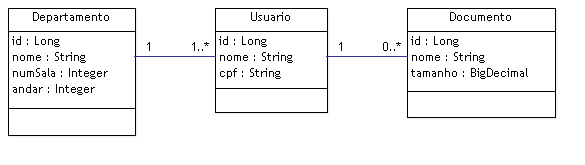
\includegraphics[scale=.8]{images/class.png} 
	 	\caption{Diagrama de classe do sistema de exemplo.}
	\end{figure} 

Após a modelagem inicial, identificamos que o sistema é divido em duas páginas:
\textbf{Página de Usuários} e \textbf{Página de Gerenciamento de Departamentos}.
Para a \textbf{Página de Usuários} temos as seguintes funcionalidades:
	\begin{itemize}
  		\item Listagem de todos os Departamentos.
  		\item Listagem de usuários para um dado departamento.
  		\item Criação/Alteração/Exclusão de usuários para um dado departamento.
  		\item Impressão de relatórios de documento associados aos usuários.
	\end{itemize}

Já para a \textbf{Página de Gerenciamento de Usuários} temos:
	\begin{itemize}
	  \item Listagem de todos os departamentos.
	  \item Criação/Alteração/Exclusão de departamentos. 
	\end{itemize}
	
Abaixo temos um esborço de como essas páginas poderiam ser implementadas:
	\begin{multicols}{2}
		\begingroup
			\centering
	 		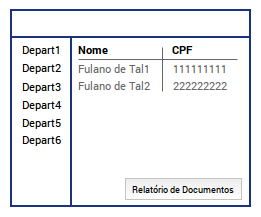
\includegraphics[scale=.7]{images/usuarioPage.png} 
	 		\captionof{figure}{Página de Usuários por Departamento.}
		\endgroup
		
		\columnbreak
		
		\begingroup
			\centering
	 		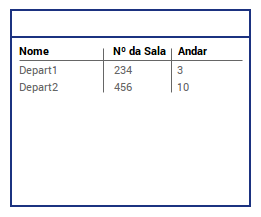
\includegraphics[scale=.7]{images/departamentoPage.png} 
	 		\captionof{figure}{Página de Gerenciamento de Departamentos.}
		\endgroup	
	\end{multicols}		
	 
\newpage
Uma forma comum de organização de \emph{managed beans} e \emph{arquivos
XHTMLs} em projeto JSF para o sistema é ilustrada no esquema abaixo:
		\begin{multicols}{2}
			
			\dirtree{%
				.1 \folder{red}{sisdep}.
				.2 \folder{red}{src/main/java}.
				.3 \folder{red}{[package]}.
				.4 \folder{red}{view}.
				.5 \folder{red}{edit}.
				.6 \folder{green}{UsuarioEditMB.java}.
				.6 \folder{green}{DocumentoEditMB.java}.
				.6 \folder{green}{DepartamentoEditMB.java}.
				.5 \folder{red}{list}.
				.6 \folder{green}{UsuarioListMB.java}.
				.6 \folder{green}{DocumentoListMB.java}.
				.6 \folder{green}{DepartamentoListMB.java}.
				.5 \folder{red}{report}.
				.6 \folder{green}{DocumentoReportMB.java}.
				}.
			  \captionof{figure}{Estrutura de Pacotes.}
		\columnbreak
			\dirtree{%
			.1 \folder{red}{sisdep}.
			.2 \folder{red}{src}.
			.3 \folder{red}{main}.
			.4 \folder{red}{webapp}.
			.5 \folder{red}{usuario}.
			.6 \folder{green}{index.xhtml}.
			.6 \folder{green}{list.xhtml}.
			.6 \folder{green}{edit.xhtml}.
			.5 \folder{red}{documento}.
			.6 \folder{green}{list.xhtml}.
			.6 \folder{green}{edit.xhtml}.
			.5 \folder{red}{departamento}.
			.6 \folder{green}{index.xhtml}.
			.6 \folder{green}{list.xhtml}.
			.6 \folder{green}{edit.xhtml}.
			.5 \folder{red}{report}.
			.6 \folder{green}{documentoReport.xhtml}.
			}.
			\captionof{figure}{Estrutura de XHTMLs.}
		\end{multicols}
		
Com a estrutura de código (tanto java quando XHTML) mostrada algumas indagações
surgem:
	\begin{enumerate}
	  	\item Apenas analisando o código fonte, quantas páginas o sistema possui? 
  		\item Quais \emph{\textbf{managed beans} e \textbf{XHTMLs}} pertencem a
  		\underline{Página de Usuários}?
  		\item E quais \emph{\textbf{managed beans} e \textbf{XHTMLs}} pertencem a
  		\underline{Página de Gerenciamento de Departamentos}?
	\end{enumerate}

Como podemos observar a resposta não parece óbivia a primeira vista e tende a se
tornar mais difícil com o aumento do número de entidades e das páginas derivadas. 
Tal dificuldade tem impacto direto no desenvolvimento tendo em vista na
dificuldade em se enxergar uma \underline{correspondência} entre os mockups e o
código resultante. A manutenção futura também é prejudicada pelo mesmo motivo.

Exposto essa problemática, vamos analizar uma outra abordagem para o
problema utilizando o \textbf{conceito de página}.
%%%%%%%%%%%%%%%%%%%%%%%%%%%%%%%%%%%%%%%%%%%%%%%%%%%%%%%%%%%%%
% 
%  Instalação 
%
%%%%%%%%%%%%%%%%%%%%%%%%%%%%%%%%%%%%%%%%%%%%%%%%%%%%%%%%%%%%% 
\section{Instalação}
Todo o código necessário para implementarmos a estuturação por páginas está
contido no projeto jbase\footnote{Para utilizar o jbase é necessário adicionar
o repositório
\emph{http://nexus.tre-pa.gov.br:8090/nexus/content/groups/public} no
\emph{pom.xml}} e é ''instalado'' no projeto adicionando a dependência no
pom.xml
	\lstinputlisting[language=XML]{snnipets/Install.xml}
%%%%%%%%%%%%%%%%%%%%%%%%%%%%%%%%%%%%%%%%%%%%%%%%%%%%%%%%%%%%%
% 
%  Convenções
%
%%%%%%%%%%%%%%%%%%%%%%%%%%%%%%%%%%%%%%%%%%%%%%%%%%%%%%%%%%%%% 
\section{Convenções e Boas Práticas}
Segue abaixo algumas convenções adotas no decorrer do documento:
	\begin{itemize}
		%%%%%%%%%%%%%%%%%%%%%%%%%%%%%%%%%%%%%%%%%%%%%%%%%%%%%%%%%%%%%
  		\item O nome do template padrão é \textbf{main.xhtml} e esta localizado no
  		diretório src/main/webapp/view/template;
		%%%%%%%%%%%%%%%%%%%%%%%%%%%%%%%%%%%%%%%%%%%%%%%%%%%%%%%%%%%%%
  		\item As \textbf{pages} estão localizadas dentro do pacote
  		src/main/java/\emph{[package]}/view/;
  		%%%%%%%%%%%%%%%%%%%%%%%%%%%%%%%%%%%%%%%%%%%%%%%%%%%%%%%%%%%%%
  		\item O pacote que contém o conteúdo (dialog, datatables e etc.) da
  		\textbf{página} é sufixado com \textbf{Page}. \emph{(ex: usuarioPage)};
		%%%%%%%%%%%%%%%%%%%%%%%%%%%%%%%%%%%%%%%%%%%%%%%%%%%%%%%%%%%%%
  		\item O managed bean controlador do template é sufixado com \textbf{PG}.
  		\emph{(ex:
  		UsuarioPG.java)};
  		 %%%%%%%%%%%%%%%%%%%%%%%%%%%%%%%%%%%%%%%%%%%%%%%%%%%%%%%%%%%%%
  		\item O managed bean controlador do template de \underline{páginas que
  		representem o conceito de gerenciamento} é sufixado com \textbf{MngtPG}.
  		\emph{(ex:
  		DepartamentoMngtPG.java)};
		%%%%%%%%%%%%%%%%%%%%%%%%%%%%%%%%%%%%%%%%%%%%%%%%%%%%%%%%%%%%%
	  	\item O arquivo XHTML que contém as definições(ui:define) da page possui o
  		nome de \textbf{index.html}
  		\item Evitar o reuso de códigos Java e XHTML entre páginas.\footnote{Com
  		esta abordagem criamos linhas independentes de código evitando conflito de
  		merges}
  		\item Incluir os componentes de dialogs (p:dialog, p:confirmDialog \ldots)
  		na região \textbf{document.body} do template.\footnote{Evita-se com isso
  		alguns bugs relacionados a componentes que precisem de \emph{overlay}}.
  		\item Nomear as classes Java para que não haja colisão entre páginas, ou
  		seja, não poderá existir duas classes chamadas
  		\textbf{\emph{departamentoTreeMB}} mesmo que estejam em pacotes diferentes.
	\end{itemize}

%%%%%%%%%%%%%%%%%%%%%%%%%%%%%%%%%%%%%%%%%%%%%%%%%%%%%%%%%%%%%
% 
%  Template Padrão
%
%%%%%%%%%%%%%%%%%%%%%%%%%%%%%%%%%%%%%%%%%%%%%%%%%%%%%%%%%%%%% 
\section{Template Padrão (main.xhtml)} 
Conforme dito anteriormente, a proposta do template padrão é de reduzir a
quantidade de templates que venham a surgir no projeto JSF. O arquivo está
localizado conforme a estrutura de diretório abaixo:
\newline
	\dirtree{%
	.1 \folder{red}{sisdep}.
	.2 \folder{red}{src}.
	.3 \folder{red}{main}.
	.4 \folder{red}{webapp}.
	.5 \folder{red}{template}.
	.6 \folder{green}{main.xhtml}.
	}
	
%%%%%%%%%%%%%%%%%%%%%%%%%%%%%%%%%%%%%%%%%%%%%%%%%%%%%%%%%%%%%
% 
%  Regiões do Template Padrão
%
%%%%%%%%%%%%%%%%%%%%%%%%%%%%%%%%%%%%%%%%%%%%%%%%%%%%%%%%%%%%% 
\subsection{Regiões do Template Padrão}
O template padrão é dividido em diversas \emph{regiões} configuráveis (que
podem ser exibidas ou não) dinâmicamente de acordo com o estrutura de cada
página.
A figura 6 ilustra graficamente as regiões do template (as regiões em cinza
representam as partes configuráveis dinamicamente):
	  
	\begin{figure}[h]   
	 	\centering
	 		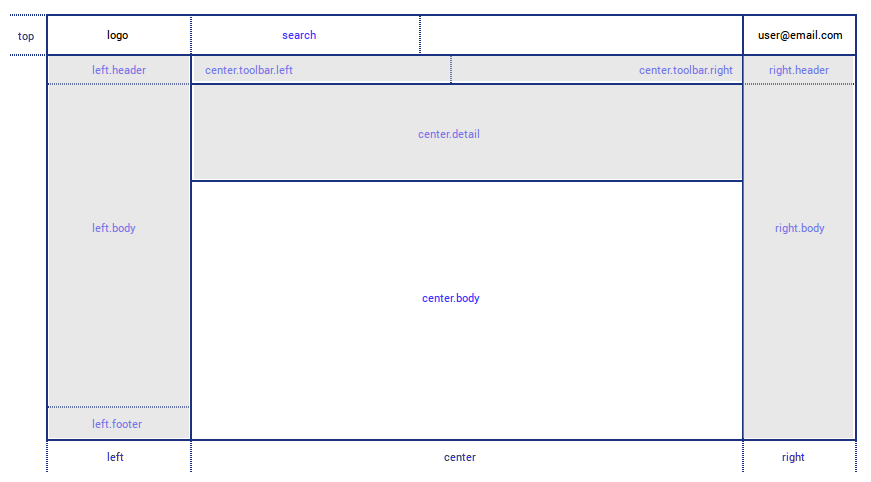
\includegraphics[scale=.6]{images/layout.png} 
	 	\caption{Regiões do template padrão}
	\end{figure}            
%%%%%%%%%%%%%%%%%%%%%%%%%%%%%%%%%%%%%%%%%%%%%%%%%%%%%%%%%%%%%	
\newpage
\subsection{Código XHTML do Template Padrão}

\lstinputlisting[language=XML]{snnipets/main.xhtml}
	\begin{itemize}
		%%%%%%%%%%%%%%%%%%%%%%%%%%%%%%%%%%%%%%%%%%%%%%%%%%%%%%%%%%%%%	
  		\item \textbf{\emph{Linha 8}} - Título da página \emph{(Nome do Sistema)}.
  		%%%%%%%%%%%%%%%%%%%%%%%%%%%%%%%%%%%%%%%%%%%%%%%%%%%%%%%%%%%%%	
  		\item \textbf{\emph{Linha 9}} - Arquivo com as definições de layout da
  		aplicação. Como a definição das \emph{regiões} do template.
		%%%%%%%%%%%%%%%%%%%%%%%%%%%%%%%%%%%%%%%%%%%%%%%%%%%%%%%%%%%%%	
  		\item \textbf{\emph{Linha 23}} - Definição a região de \textbf{''top''} da
  		aplicação
  		\item \textbf{\emph{Linha 24}} - Inclui o trecho XHTML do topo.
  		\item \textbf{\emph{Linha 38}} - Define a região \textbf{''left.header''} do
		template.
		\item \textbf{\emph{Linha 44}} - Define a região \textbf{''left.body''} do
		template.
		\item \textbf{\emph{Linha 49}} - Define a região \textbf{''left.footer''} do
		template.
		\item \textbf{\emph{Linha 68}} - Define a região \textbf{''center.toolbar.left''}
		do template.
		\item \textbf{\emph{Linha 72}} - Define a região \textbf{''center.toolbar.right''}
		do template.
		\item \textbf{\emph{Linha 79}} - Define a região \textbf{''center.detail''} do
		template.
		\item \textbf{\emph{Linha 85}} - Define a região \textbf{''center.body''} do
		template.
		\item \textbf{\emph{Linha 97}} - Define a região \textbf{''right.header''} do
		template.
		\item \textbf{\emph{Linha 102}} - Define a região \textbf{''right.body''} do
		template.
		\item \textbf{\emph{Linha 108}} - define a região \textbf{''document.body''}
		do template. Esta região deverá ser usada nos ''\emph{indexs}'' quando existir a
		necessidade de se incluir algum componente diretamente no \emph{body}.
		\item \textbf{\emph{Linha 111}} - Growl \underline{padrão} para informções do
		sistema.
		\item \textbf{\emph{Linha 114 a 123}} - Trecho XHTML do dialog de erro
		\underline{padrão} do sistema.
	\end{itemize}
%%%%%%%%%%%%%%%%%%%%%%%%%%%%%%%%%%%%%%%%%%%%%%%%%%%%%%%%%%%%%
% 
%  Conceito de Página
%
%%%%%%%%%%%%%%%%%%%%%%%%%%%%%%%%%%%%%%%%%%%%%%%%%%%%%%%%%%%%% 
\section{Conceito de Página}
De maneira direta, uma página é definida como \textbf{ todo o conteúdo xhtml que se
mantém sob uma mesma URL} (mantém o scopo de visão do JSF), ou seja, todos os
componentes do Primefaces (dialogs, datatables, datalists etc.) utilizados para
montar um index (xhtml que \emph{extende} o template padrão) pertencem a uma
página.

De posse deste conceito, é proposto que a organização do código java e
xhtml necessário para montar uma página seja agrupado de forma coerente.
%%%%%%%%%%%%%%%%%%%%%%%%%%%%%%%%%%%%%%%%%%%%%%%%%%%%%%%%%%%%%
% 
%  Organização das Páginas
%
%%%%%%%%%%%%%%%%%%%%%%%%%%%%%%%%%%%%%%%%%%%%%%%%%%%%%%%%%%%%% 
\subsection{Organização das Páginas}
As seções a seguir mostram a forma de organização dos códigos Java e XHTML.
Para tanto, tomemos como exemplo a entidade \emph{Usuário} que conceitualmente
representa uma página do sistema.
Para esta entidade iremos criar uma página onde irá conter a listagem de usuários, o dialog de
edição de usuários e qualquer outro elemento que faça parte da estrurua que
forma a página.
%%%%%%%%%%%%%%%%%%%%%%%%%%%%%%%%%%%%%%%%%%%%%%%%%%%%%%%%%%%%%
% 
%  Organização da Página de Usuário - Parte Java 
%
%%%%%%%%%%%%%%%%%%%%%%%%%%%%%%%%%%%%%%%%%%%%%%%%%%%%%%%%%%%%% 
\subsubsection{Organização da Página de Usuários}
\label{org-pg-user} Na estrutura de código Java a forma mais adequada para organizarmos os códigos
java é através de \underline{\emph{pacotes}}. De acordo com as funcionalidades
elencadas na seção de introdução deste documento daremos o nome para o pacote da
\textbf{Página de Usuários} de \emph{usuarioPage}. Em seguida criamos uma classe
java chamada \emph{UsuarioPG.java} que irá gerenciar todos os aspectos referente
a página e ,além disso, iremos trazer para este novo pacote(\emph{usuarioPage})
os managed beans correpondentes.

Na parte XHTML é criado um diretório com o mesmo nome do pacote em java
(usuarioPage) e o arquivo que gerencia a página é chamado de
index.xhtml\footnote{Este é o arquivo que extende e possui todos os
''\emph{defines}'' do  template padrão main.xhtml.} 

Como resultado teremos a seguinte estrutura: 
	\begin{multicols}{2}
		\dirtree{%  
		.1 \folder{red}{sisdep}.
		.2 \folder{red}{src/main/java}.
		.3 \folder{red}{[package]}.
		.4 \folder{red}{view}.
		.5 \folder{red}{usuarioPage}.
		.6 \folder{green}{UsuarioPG.java}.
		.6 \folder{green}{UsuarioEditDialogMB.java}.
		.6 \folder{green}{UsuarioListMB.java}.
		.6 \folder{green}{DocumentoReportMB.java}.
		.6 \folder{green}{DepartamentoTreeMB.java}.
		}.
		\captionof{figure}{Estrutura de de pacotes.}
		\columnbreak
		
		\dirtree{%
		.1 \folder{red}{sisdep}.
		.2 \folder{red}{src}.
		.3 \folder{red}{main}.
		.4 \folder{red}{webapp}.
		.5 \folder{red}{view}.
		.6 \folder{red}{usuarioPage}.
		.7 \folder{green}{index.xhtml}.
		.7 \folder{green}{usuarioEditDialog.xhtml}.
		.7 \folder{green}{usuarioList.xhtml}.
		.7 \folder{green}{departamentoTree.xhtml}.
		}.
		\captionof{figure}{Estrutura de diretórios.}
	\end{multicols}
Com isso, qualquer \emph{managed bean} pertencente a \underline{página de
usuários} estará contido dentro do pacote \textbf{view.usuarioPage} e qualquer
componente XHTML estará contido no diretório \textbf{/view/usuarioPage}

%%%%%%%%%%%%%%%%%%%%%%%%%%%%%%%%%%%%%%%%%%%%%%%%%%%%%%%%%%%%%
% 
%  Organização da Página de Gerenciamento de Departamentos 
%
%%%%%%%%%%%%%%%%%%%%%%%%%%%%%%%%%%%%%%%%%%%%%%%%%%%%%%%%%%%%% 
\subsubsection{Organização da Página de Gerenciamento de Departamentos}
Utilizado o mesmo raciocínio do seção \ref{org-pg-user} devemos criar um
pacote para a guardar o conteúdo da \textbf{Página de Gerenciamento de
Departamentos}. Como o página é uma página de \underline{gerenciamento} o nome
do pacote resultante será: \emph{\textbf{departamentoMngtPage}}

Na parte XHTML é criado um diretório com o mesmo nome do pacote em java
(departamentoMngtPage) e o arquivo que gerencia a página é chamado de
index.xhtml. 

Como resultado teremos a seguinte estrutura: 
	\begin{multicols}{2}
		\dirtree{%
		.1 \folder{red}{sisdep}.
		.2 \folder{red}{src/main/java}.
		.3 \folder{red}{[package]}.
		.4 \folder{red}{view}.
		.5 \folder{red}{departamentoMngtPage}.
		.6 \folder{green}{DepartamentoMngtPG.java}.
		.6 \folder{green}{DepartamentoMngtEditDialogMB.java}.
		.6 \folder{green}{DepartamentoMngtListMB.java}.
		}.
		\captionof{figure}{Estrutura de de pacotes.}
		
		\columnbreak
		
		\dirtree{%
			.1 \folder{red}{sisdep}.
			.2 \folder{red}{src}.
			.3 \folder{red}{main}.
			.4 \folder{red}{webapp}.
			.5 \folder{red}{view}.
			.6 \folder{red}{departamentoMngtPage}.
			.7 \folder{green}{index.xhtml}.
			.7 \folder{green}{departamentoMngtEditDialog.xhtml}.
			.7 \folder{green}{departamentoMngtList.xhtml}.
			}.
		 \captionof{figure}{Estrutura de diretórios.}
	\end{multicols}

Como podemos perceber, apesar de utilizarmos o nome da entidade para criarmos o
nome do pacote na seção \ref{org-pg-user} (\emph{usuarioPage}) aqui neste
exemplo definimos o nome como \emph{departamentoMngtPage} que representa  o
conceito lógico (Gerenciar Departamento), ou a finalizade da página em si, que
dá o nome do pacote correspondente.
%%%%%%%%%%%%%%%%%%%%%%%%%%%%%%%%%%%%%%%%%%%%%%%%%%%%%%%%%%%%%
% 
%  Código Java da Página de Usuário (UsuarioPG.java)
%
%%%%%%%%%%%%%%%%%%%%%%%%%%%%%%%%%%%%%%%%%%%%%%%%%%%%%%%%%%%%% 
\subsection{Código Java da Página de Usuário (UsuarioPG.java)}
Conforme dito em seções anteriores, umas das vantagens da utilização do Template
Padrão é a flexibilidade de configuração das regiões de acordo com o layout
definido pela equipe de design. A forma como esta configuração é feita é
ilustrada pela seguinte alteração no código da página a seguir:
	\lstinputlisting{snnipets/UsuarioPG-UILayout.java}
		\begin{itemize}
		  \item \textbf{\emph{Linha 17}} - Injeção da classe \emph{UILayout} que é
		  responsável por manipular o template padrão.
		  \item \textbf{\emph{Linha 21}} - Método da classe \emph{UILayout} que define
		  se uma região do template padrão é renderizada ou não. No exemplo desta
		  linha a região \textbf{''left''} do template é setada para ser renderizada. 
		  \item \textbf{\emph{Linha 22}} - Define que a região \textbf{''right''} do
		  template padrão \textbf{não} é renderizada.
		  \item \textbf{\emph{Linha 23}} - Define que a região
		  \textbf{''center.detail''} do template padrão é renderizada.
		\end{itemize}

Como resultado do código acima temos o seguinte layout:
	\begin{figure}[h]
		\centering
	 	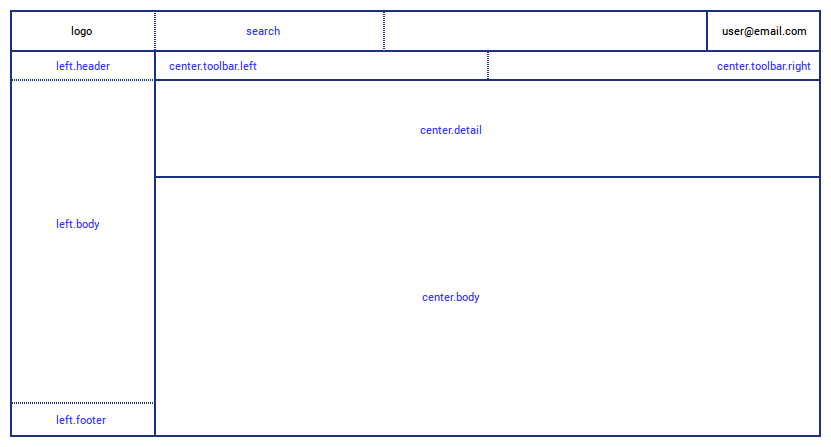
\includegraphics[scale=.6]{images/layoutUsuarioPage.png} 
	 	\caption{Layout da Página de Usuários.}
	\end{figure} 
%%%%%%%%%%%%%%%%%%%%%%%%%%%%%%%%%%%%%%%%%%%%%%%%%%%%%%%%%%%%%
% 
% Código XHTML da Página de Usuários (usuarioPage/index.xhtml)
%
%%%%%%%%%%%%%%%%%%%%%%%%%%%%%%%%%%%%%%%%%%%%%%%%%%%%%%%%%%%%% 
\newpage
\subsection{Código XHTML da Página de Usuários (usuarioPage/index.xhtml)}
Abaixo temos um exemplo de um código xhtml de uma página de \emph{index} vazia.
No momento esta possui apenas as definições(\emph{ui:define}) das regiões
definidas(\emph{ui:insert}) no template padrão(\emph{main.xhtml}). Caso alguma
seção(\emph{ui:define}) não seja utilizada, esta pode ser deletada do arquivo de
\emph{index.xhtml} sem maiores problemas.
	\lstinputlisting[language=XML]{snnipets/index-usuarioPage.xhtml} 
		\begin{itemize}
  			\item \textbf{\emph{Linha 4}} - Atributo \emph{template} da tag
  			\textbf{\emph{ui:composition}} que define qual atributo o xhtml irá
  			utilizar.
  			\item \textbf{\emph{Linha 7}} - Definição da região
  			\textbf{''left.header''} do template.
  			\item \textbf{\emph{Linha 11}} - Definição da região \textbf{''left.body''}
  			do template. É nesta região que usualmente se encontra a listagem em árvore
  			(\emph{p:tree}) da página.
  			\item \textbf{\emph{Linha 15}} - Define a região \textbf{''left.footer''}
  			do template. É nesta região que usualmente se encontra a totalização de itens
  			que se encontram na listagem em árvore.
  			\item \textbf{\emph{Linha 19}} - Define a região
  			\textbf{''center.toolbar.left''} do template. É nesta região que é inserido
  			os \emph{buttons} no lado esquerdo da barra de ferramentas. 
  			\item \textbf{\emph{Linha 23}} - Define a região
  			\textbf{''center.toolbar.right''} do template. É nesta região que é
  			inserido os \emph{buttons} no lado direito da barra de ferramentas.
  			\item \textbf{\emph{Linha 27}} - Define a região \textbf{''center.detail''}
  			do template.
  			\item \textbf{\emph{Linha 31}} - Define a região \textbf{''center.body''}
  			do template.
  			\item \textbf{\emph{Linha 35}} - Define a região \textbf{''document.body''}
  			do template.
		\end{itemize}

%%%%%%%%%%%%%%%%%%%%%%%%%%%%%%%%%%%%%%%%%%%%%%%%%%%%%%%%%%%%%
% 
%  Código Java da Página de Genreciamento de Departametos
% (DepartamentoMngtPG.java)
%
%%%%%%%%%%%%%%%%%%%%%%%%%%%%%%%%%%%%%%%%%%%%%%%%%%%%%%%%%%%%% 	
\subsection{Código Java da Página de Genreciamento de Departametos
(DepartamentoMngtPG.java)} 
	\lstinputlisting{snnipets/DepartamentoMngtPG-UILayout.java}
Como resultado do código acima temos o seguinte layout:
	\begin{figure}[h]
		\centering
	 	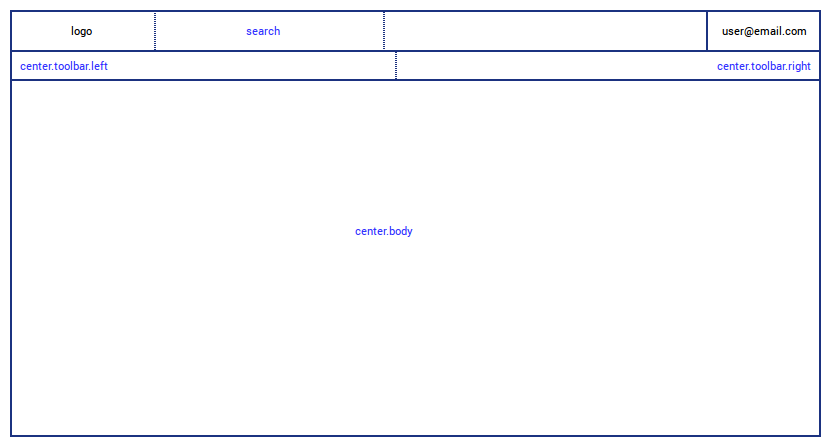
\includegraphics[scale=.6]{images/layoutDepartamentoMngtPage.png} 
	 	\caption{Layout da Página de Gerenciamento de Departamentos.}
	\end{figure}
	
%%%%%%%%%%%%%%%%%%%%%%%%%%%%%%%%%%%%%%%%%%%%%%%%%%%%%%%%%%%%%
% 
% Código XHTML da Página de Usuários (departamentoMngtPage/index.xhtml)
%
%%%%%%%%%%%%%%%%%%%%%%%%%%%%%%%%%%%%%%%%%%%%%%%%%%%%%%%%%%%%% 
\newpage
\subsection{Código XHTML da Página de Genreciamento de Departametos
(departamentoMngtPage/index.xhtml)} 
\lstinputlisting[language=XML]{snnipets/index-departamentoMngtPage.xhtml} 
%%%%%%%%%%%%%%%%%%%%%%%%%%%%%%%%%%%%%%%%%%%%%%%%%%%%%%%%%%%%%
% 
%  Reescrevendo URLs com Pretty-Faces
%
%%%%%%%%%%%%%%%%%%%%%%%%%%%%%%%%%%%%%%%%%%%%%%%%%%%%%%%%%%%%% 
\section{Reescrevendo URLs com Pretty-Faces}
O projeto \emph{pretty-faces}  apesar de possuir o ''faces'' na sua
nomenclatura, não possui nenhum componente visual para utilizarmos em projetos
JSF. Seu objetivo principal é \underline{reescrever as URLs} do JSF tornado-as
''amigáveis'' para o usuário final sem a necessidade de renomearmos ou
reestruturarmos os diretórios onde se encontram os XHTMLs da aplicação.
%%%%%%%%%%%%%%%%%%%%%%%%%%%%%%%%%%%%%%%%%%%%%%%%%%%%%%%%%%%%%
% 
%  Instalação
%
%%%%%%%%%%%%%%%%%%%%%%%%%%%%%%%%%%%%%%%%%%%%%%%%%%%%%%%%%%%%% 
\subsection{Instalação}
Para se instalar o Pretty-Faces é apenas necssário a inclusão da respectiva
dependência no \emph{pom.xml} conforme abaixo:
	\lstinputlisting[language=XML]{snnipets/Install-Pretty-Faces.xml}

Após a instalação, todo o processo de mapeamento de URLs do pretty-faces estará
concentrado no arquivo \emph{\textbf{pretty-faces.xml}} localizado na estrutura
de diretório conforme a seguir:
	\newline
		\dirtree{%
		.1 \folder{red}{sisdep}.
		.2 \folder{red}{src}.
		.3 \folder{red}{main}.
		.4 \folder{red}{webapp}.
		.5 \folder{red}{WEB-INF}.
		.6 \folder{green}{pretty-faces.xml}.
		}.
\newpage
\subsection{Mapeamento de Páginas no Pretty-Faces}
O trecho de código abaixo exibe a forma de como é realizado o mapeamento dentro
do arquivo \emph{\textbf{pretty-faces.xml}}:
	\lstinputlisting[language=XML]{snnipets/Pretty-Faces.xml}
		\begin{itemize}
  			\item \textbf{\emph{Linha 5}} - ID do mapeamento do pretty-faces. Deve ser
  			único no arquivo.
  			\item \textbf{\emph{Linha 6}} - Define o padrão da URL que será
  			exposta para o usuário final. É esta URL que deverá ser indicada no navegador para
  			acessar a página correspondente.
  			\item \textbf{\emph{Linha 7}} - Caminho a partir do diretório
  			\emph{src/main/webapp} do arquivo XHTML correspondente a página.
  			\item \textbf{\emph{Linha 8}} - É nesta linha que a chamada do metodo load
  			da página correspondente, ou seja, caso a URL digitada no navegador seja
  			\emph{http://sisdep/usuarios} o método \emph{load} é
  			invocado. 
  			\item \textbf{\emph{Linha 14 a 18}} - Definições para a Página de
  			Gerenciamento de Departamentos
		\end{itemize} 

A cada nova página do sistema um novo bloco \emph{''url-mapping''} deverá ser
definido com os dados da respectiva página.

\section{Conclusão}
Com a abordagem explicada anteriormente podemos elencar os seguintes ganhos:
	\begin{enumerate}
 		\item Criação de uma relação consistente e direta entre o código Java e XHTML
 		facilitando a visualização em código do conteúdo de cada página.
 		\item Flexibilidade na criação de templates.
 		\item Utilização consistente do escope de visão (\emph{@ViewScope}).
 		\item Melhor estruturação do código fonte.
	\end{enumerate}

\end{document}
